\documentclass[twocolumn,9pt]{article}
%\documentclass[9pt]{article}
%\documentclass[../main.tex]{subfiles}
\usepackage{amsmath}
\usepackage{amssymb}
\usepackage{graphicx}
\usepackage{amsthm}
\usepackage{breqn}
\usepackage{float}
\usepackage{enumerate}
\usepackage{comment}

\newcommand\norm[1]{\lVert#1\rVert}
\newtheorem{theorem}{Theorem}[section]
\newtheorem{corollary}{Corollary}[theorem]
\newtheorem{proposition}{Proposition}[theorem]
\newtheorem{lemma}[theorem]{Lemma}
\theoremstyle{definition}
\newtheorem{definition}{Definition}[section]
\theoremstyle{remark}
\newtheorem*{remark}{Remark}

%\begin{figure}
%\includegraphics[width=1.0\textwidth]{plt_introduction.pdf}
%\caption{Two paths having small Euclidean distance, but big Signature
%            difference}
%\includegraphics[scale=0.5]{plt_introduction.pdf}
%\centering
%\end{figure}

\title{The Signature Transform for Time Series Classification (beta.1)}
\author {-}

\begin{document}

\maketitle
\begin{section}{Introduction}
The purpose of this paper is to propose a way to use the 
\emph{signature transform} as a supporting tool for 
the classification of time series.


We suppose to have a dataset 
$\mathcal{D} = \{ \hat{x}_i, y_i \}_{i=1, \dots , N}$
of $N$ samples such that
each "point" $\hat{x}_i$ is
an array of ordered real numbers coming from measurements,
with associated \emph{labels} $y_i$ with values $0$ or $1$.

Examples are ubiquitous.
For instance, $\hat{x}_i$ can be the temperature during some day $i$
monitored every minute, with $y_i$ positive
if a specific meteorological
phenomenon happened. Or in medical applications, $\hat{x}_i$ can be
the hearth rate of a patient while $y_i$ a flag for the presence of a pathology.
In a completely different context,
the measurements can be seen as financial transactions
and the labels used to mark cases of fraud.


In our setting, the measurements $\hat{x}_i$
are allowed to have different lengths.
This makes the use of standard algorithms a bit harder,
since pointwise comparisons (and therefore common norms)
cannot be directly used.
On the other hand, we explain how by using the signature transform 
we are able to bypass this inconvenience, ultimately \emph{compressing}
every sample $\hat{x}_i$ into a new array $\hat{p}_i$
of a controllable length.
This length turns out to be \emph{constant} for every $i$.
On this new preprocessed 
dataset $\{ \hat{p}_i, y_i\}_{i = 1, \dots, N}$,
we finally perform the classification task using the common KNN algorithm,
possible because the samples are now of equal shape.


In the first part we revise the definition 
of the signature transform, 
an object coming from  stochastic analysis
(\cite{FrizVic}, \cite{LyonsBook}).
Our approach is direct and concise, with minimal definitions
and especially for readers (possibly with a limited mathematical background)
who desire to see if the approach can actually offer enough advantages
before moving into the theory in a later step.
The resource \cite{PRIMER} expands our exposition and 
is particularly recommended.

In the second half we perform classification experiments involving
curves of familiar shapes (segments, sinusoids, impulses), commenting
benefits and limits of the proposed methodology.
\end{section}


\begin{section}{The Signature Transform}
Let $f: [0, 1] \to \mathbb{R}$ be a smooth function starting from $0$,
intuitively representing the data that we measure.
Since it is important to keep track of time, we consider its
\emph{augmentation} $X(t) = (t, f(t))$.
We indicate with $X^1(t)$ the first component of $X$, in this case
$t$, while with $X^2(t)$ the component $f(t)$.
Before proceeding, we need to revise some elementary combinatorics.

\begin{definition}[Multi-index]
A multi-index $I$ of depth $n \geq 1$ is an ordered collection of $n$ digits,
$I = (i_1, \dots, i_n)$, each digit being $1$ or $2$.
\end{definition}
For each depth $n$, we have $2^n$ possible multi-indices.
For instance, if we consider \emph{all} the indices until depth 4,
we obtain a total of $\sum_{i=1}^4 2^i = 30$ coefficients.

\begin{definition}[Canonical simplex]
The $d$-dimensional canonical simplex is the set:
\begin{equation*}
\Delta^d = \{ (u_1, \dots, u_d), u_i \in [0,1] ,
            0 < u_1 < \cdots < u_d < 1 \}
\end{equation*}
\end{definition}

We are now ready to introduce the main object.
\begin{definition}[Signature coefficient]
The signature coefficient corresponding to the multi-index
$I_n = (i_1, \dots, i_n)$
is the real number $s_{I_n}$ defined as:
\begin{equation}
s_{I_n} = \int_{\Delta^n} \dot{X}^{i_1}(u_1) \cdots
                            \dot{X}^{i_n}(u_n) du_1 \cdots du_n
\end{equation}
where $\dot{X}^k$ is the derivative of the $k$-th component of the path $X$.
\end{definition}

Since in our case we consider only paths of the form
$X = (t, f(t))$, the integrands are always mixed products of derivatives
$f'(t)$. Considering all the possible combinations gives rise to the Signature
Transform.

\begin{definition}[The Signature Transform]
The \emph{signature transform} $S(X)$ is the infinite, 
ordered collection of all the possible
signature coefficients. The truncated
signatures $S^N(X)$ is instead the collection of all the
coefficients until depth $N$, included.
\end{definition}


For instance, $S^4(X)$ is a collection of $30$ real numbers.
We do not spend more time concerning the theoretical aspects,
but the reader should be aware of the existence of a vast literature,
including extensions to the multi-dimensional case, random paths
and connections to more general types of differential equations.

\begin{comment}
Comparisons with the integral Taylor expansion 
are also possible
(\cite{KPS}, chapter 2.3).

Given two paths $g$ and $f$, we have
$S((t, g(t))) = S((t, f(t))$ if and only if $f = g$.
Therefore when transforming our data, there is no theoretical risk of
losing information. 
But on the other hand, since we in practice can only compute
$S^K(X)$ until a certain depth, the previous equality is no more guaranteed.
It can theoretically happen to have two different paths sharing the same
\emph{truncated} signature up to a level. It is here that the limits
our methodology are encountered.
\end{comment}
\end{section}


\begin{section}{Methodology}

\begin{subsection}{Generating data}
We suppose that every sequence of measurements comes from
a smooth function $f: [0, 1] \to \mathbb{R}$ evaluated on a finite
number of nodes. Timestamps are added in the second coordinates.

For instance, if $3$ consecutive measurements $v_0, v_1, v_2$ are taken,
we store them as an array of couples $((v_0, 0), (v_1, 0.5), (v_2, 1))$.
If instead $5$ measurements are stored, but the third is lost,
the array will be $((v_0, 0), (v_1, 0.25), (v_3, 0.75), (v_4, 1))$.

It is important to point out how we always assume to work in the time
interval $[0, 1]$, therefore data stored in other time formats must be 
rescaled to match this model hypothesis. Furthermore it is also recommended
to perform translations so to make every array in the dataset
to start with $v_0 = 0$.
If these remarks are followed,
the signature transform is guaranteed to be injective and therefore 
we reduce the risk of losing information during the conversion.


We consider a total of three experiments,
always with datasets of $400$ time series,
each of random length from $2$ to $100$.
The labels $0$ and $1$, as well as the function $f$ 
 are specified under the corresponding sections.
The "exact" generated time series
are always perturbed with Gaussian noises ($\sigma = 0.01$)
and $10\%$ of its points are randomly removed
(for a minimum final length of two measurements).
\end{subsection}


\begin{subsection}{Computing the Signature}
Every array described as in the previous section is ready to
be used as parameter for the \emph{signatory} Python library 
(\cite{Signatory}).
We choose to stop at depth 4, therefore every path is converted to
an array of length $30$ 
\emph{independently of its starting size}.
\end{subsection}

\begin{subsection}{Classifying the time series}
The new dataset of $400$ samples of length $30$ is randomly shuffled,
split into $50$-$50$ for training and validation,
and finally the 
KNN method is used to perform the classification task on
$14 \approx \sqrt{200}$ neighbors. 
\end{subsection}

\begin{subsection}{Meaning of the plots}
For each case of study three plots are attached.
The first shows three randomly selected curves from the original dataset,
in order to provide a visual support.
Different colors correspond to different labels.


The second plot displays the signatures of these three paths.
Is it therefore a collection of $30$ real numbers 
ordered on the x-axis. From an intuitive viewpoint,
if the signatures observed for the two classes are
\emph{typically} different, we expect the classification to be more
successful.


The third plot is a way to visualize in 2d the whole transformed dataset.
The signatures of our data, originally of dimension $30$, are here
plotted in dimension 2 by using the 
\emph{Multidimensional Scaling} method, commonly abbreviated MDS, so that
distances between the paths, here measured as the euclidean norm between
their signatures, are preserved. Paths represented with a black star
are misclassified. 
\end{subsection}
\end{section}


\begin{section}{Straight lines}
The paths generated in this dataset follow the simple equation
\begin{equation}
	f(t) = at
\end{equation}
for a coefficient $a \in \mathbb{R}$. For every time series
the coefficient $a$ is randomly uniformly selected between $-1$ and
$1$. Positive cases are labeled with $1$, negative cases with $0$.
We are simply classifying segments according to their
positive or negative slope.

\begin{figure}[H]
\center
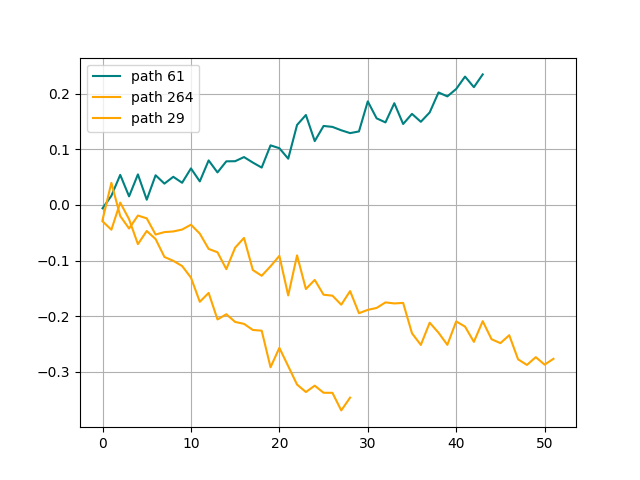
\includegraphics[width=0.28\textwidth]{proposed_plots/SEG-paths-seed0.png}
\caption{
Thee different samples from the first dataset.
We can see that they have been perturbed by the noise
and have different lengths.
}
\end{figure}

\begin{figure}[H]
\center
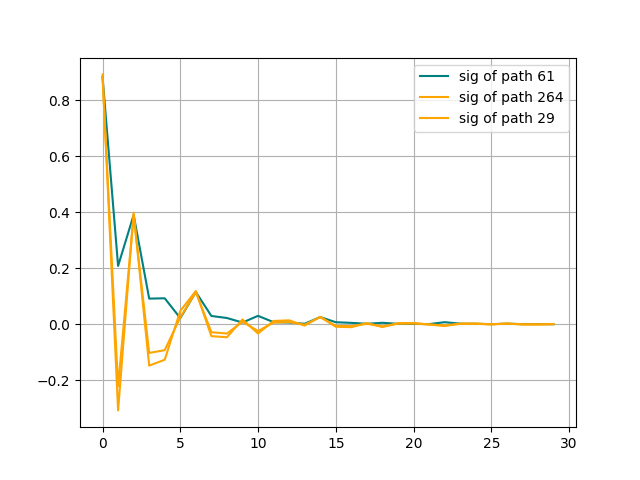
\includegraphics[width=0.30\textwidth]{proposed_plots/SEG-signatures-seed0.png}
\caption{
The signature coefficients of the paths before,
computed up to level 4.
We can already see a remarkable difference between the two classes,
therefore we expect good classification results on this converted dataset.
}
\end{figure}

When running the KNN algorithm on the preprocessed dataset, the following
results are available, suggesting a clear success:

\begin{tabular}{ |c|c| }
\hline
Training Accuracy & Validation Accuracy \\
99\%	& 99\%	\\
\hline
\end{tabular}

\begin{figure}[H]
\center
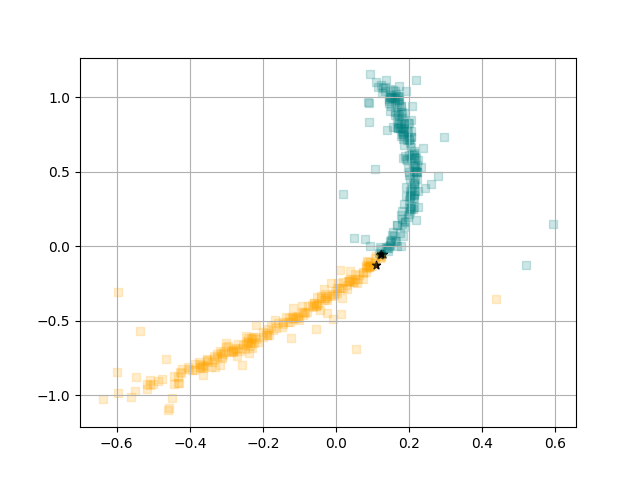
\includegraphics[width=0.40\textwidth]{proposed_plots/SEG-isometry-seed0.png}
\caption{
All the signatures, each corresponding to a single time series,
are finally plot in 2d using the MDS classic algorithm.
We can spot e very regular geometric shape, with misclassified points
lying at the boundary.
}
\end{figure}

\end{section} % ending straight lines

\begin{section}{Sinusoids}
The paths in this dataset follow the equation:
\begin{equation}
f(t) = \sin(2 \pi k)
\end{equation}
For each time series, the integer $k$
is randomly sampled between 1, 2, 3 or 4.
A label of $0$ is assigned for the cases $k = 0, 1$,
and a label of $1$ otherwise.


When running the KNN algorithm on the preprocessed dataset, the following
results are available, suggesting a success:

\begin{tabular}{ |c|c| }
\hline
Training Accuracy & Validation Accuracy \\
95\%	& 97\%	\\
\hline
\end{tabular}


\begin{figure}[H]
\center
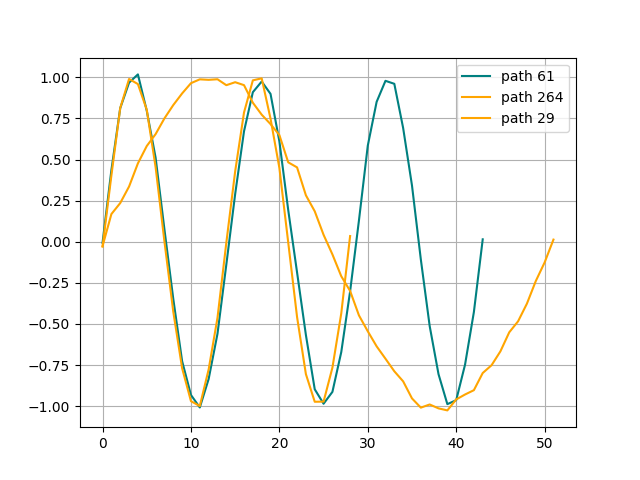
\includegraphics[width=0.30\textwidth]{proposed_plots/SIN-paths-seed0.png}
\caption
{
Three different noised sinusoids from the second dataset.
We can see the differences in frequencies and lengths.
}
\end{figure}

\begin{figure}[H]
\center
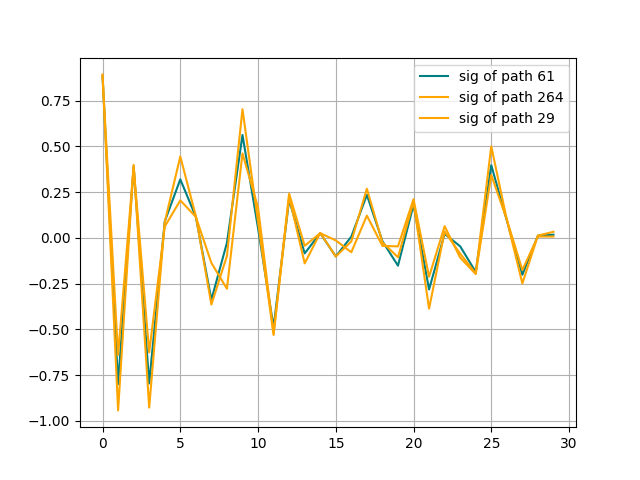
\includegraphics[width=0.31\textwidth]{proposed_plots/SIN-signatures-seed0.png}
\caption{
The signature coefficients of the paths before,
computed up to level 4.
The differences between the classes
are less remarkable when compared to the previous example.
}
\end{figure}

\begin{figure}[H]
\center
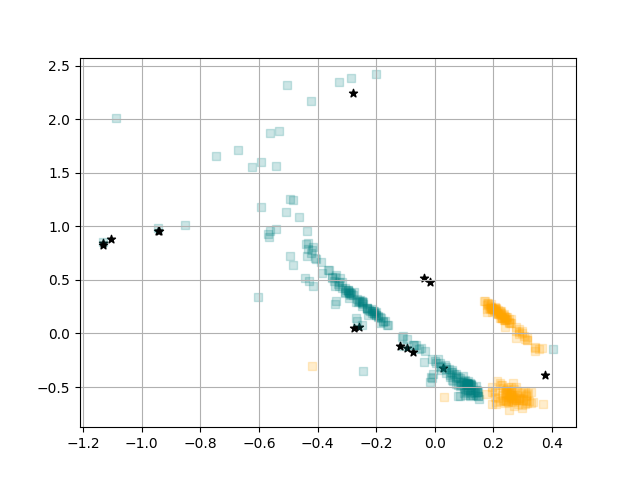
\includegraphics[width=0.35\textwidth]{proposed_plots/SIN-isometry-seed0.png}
\caption{
All the signatures
are finally plot in 2d using the MDS classic algorithm.
We can spot e very nice geometric shape. Misclassified points
are this time a harder to interpret.
}
\end{figure}

\end{section} % ending sinusoids

\begin{section}{Impulses}
The paths in this dataset follow the equation:
\begin{equation}
f(t) = e^{ - \frac{(t - p)^2}{0.01^2}}
\end{equation}
For each time series,
the value of $p$ is randomly uniformly sampled in $[0.2, 0.8]$.
Labels $0$ correspond to $p < 0.5$, and labels $1$ otherwise.

\begin{figure}[H]
\center
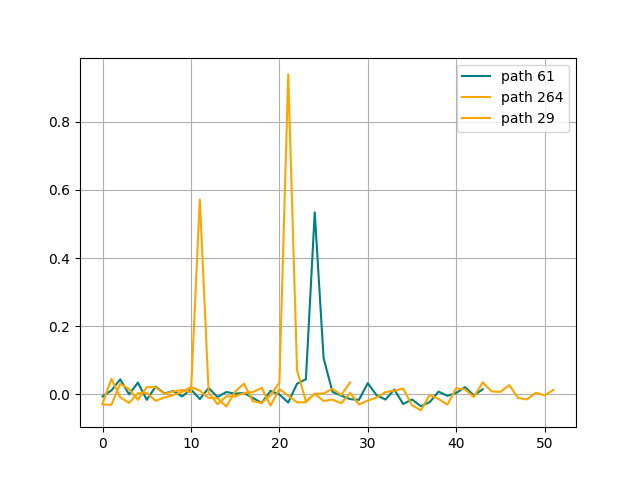
\includegraphics[width=0.35\textwidth]{proposed_plots/IMP-paths-seed0.png}
\caption{
Three different noised impulses from the third dataset,
differing mainly for the position of the peak.
}
\end{figure}

\begin{figure}[H]
\center
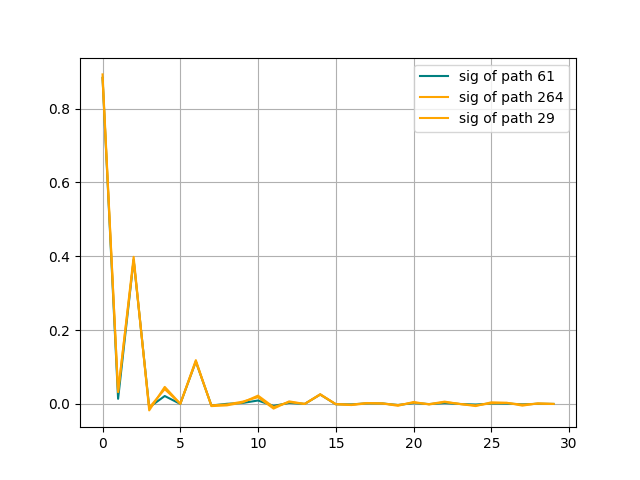
\includegraphics[width=0.35\textwidth]{proposed_plots/IMP-signatures-seed0.png}
\caption{
The signature coefficients of the paths before,
computed up to level 4.
This time is harder to properly spot the difference between the two classes.
A further analysis (here not reported) reveal how the
signatures are all very similar, with small differences
caused by the peaks locations.
}
\end{figure}

When running the KNN algorithm on the preprocessed dataset, the following
results are available, suggesting a moderate success:

\begin{tabular}{ |c|c| }
\hline
Training Accuracy & Validation Accuracy \\
82\%	& 77\%	\\
\hline
\end{tabular}

\begin{figure}[H]
\center
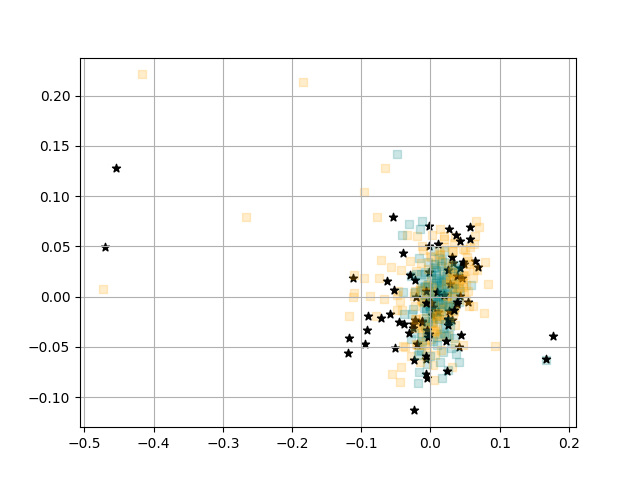
\includegraphics[width=0.35\textwidth]{proposed_plots/IMP-isometry-seed0.png}
\caption{
All the signatures, each corresponding to a single time series,
are finally plot in 2d using the MDS classic algorithm.
On the one hand we can spot a very regular shape,
on the other hand it is hard to understand the reason for
misclassification.
Maybe a 3d representation
could make the interpretation easier.
}
\end{figure}

\end{section}


\begin{section}{Conclusions}
Classifying time series is always a challenging task, especially when
working with data of different lengths.
Preprocessing with the signature transform allows to compress
them into a new database of a fixed regular shape,
on which classical algorithms like KNN can be successfully used.

We checked this strategy with the three cases of common use,
obtaining experimentally good accuracy values.
Therefore, we see in this methodology a potential for further applications.
\end{section}


\bibliographystyle{alpha} % alternative is "plain" reference style
\bibliography{./references/thebibliography}
\end{document}
